\documentclass[aspectratio=169]{beamer}
   \usetheme{metropolis}
   \setbeamertemplate{blocks}[rounded][shadow=false]
\usepackage{url}
\usepackage{hyperref}
\usepackage{booktabs}
\usepackage{tabularx}
\usepackage{dcolumn}
   \newcolumntype{d}[1]{D{.}{.}{#1}}
\usepackage{graphicx}
\usepackage[justification=raggedright]{caption}
\usepackage{adjustbox}
\usepackage{color}
\usepackage{textpos}
\usepackage{etoolbox}
\usepackage[cache=true,cachedir=minted_cache]{minted}
\usepackage{multimedia}
\usepackage{comment}

\captionsetup[figure]{justification=centering}

\makeatletter
\patchcmd{\beamer@sectionintoc}{\vskip1.5em}{\vskip0.5em}{}{}
\makeatother

\definecolor{smured}{rgb}{0.797,0,0.027}
\definecolor{smublue}{RGB}{48,64,116}
\definecolor{dkgreen}{rgb}{0,0.6,0}
\definecolor{gray}{rgb}{0.5,0.5,0.5}
\definecolor{mauve}{rgb}{0.58,0,0.82}
\definecolor{text_gray}{RGB}{46,58,62}

\setbeamercolor{progress bar}{fg=smured,bg=smublue}
\setbeamercolor{title separator}{fg=smublue}
\setbeamercolor{frametitle}{bg=smublue}

\metroset{
  numbering=fraction
}

\hypersetup{
  colorlinks=true,
  allcolors=text_gray,
  urlcolor=smured,
}

\addtobeamertemplate{frametitle}{}{
\begin{textblock*}{1cm}(\textwidth,-0.96cm)

\includegraphics[width=0.9cm]{images/smu_logo.pdf}
\end{textblock*}}

\setminted{breaklines,linenos,fontsize=\scriptsize}
\setmintedinline{fontsize=auto}

\title{Containerizing All the Things: Using Containers for Research}
\author{Robert Kalescky\\HPC Research Scientist\\Adjunct Professor of Data Science}
\institute{
Research Technology Services\\
Office of Information Technology\\
Southern Methodist University}
\date{}

\begin{document}

\begin{frame}
\titlepage
\end{frame}

\begin{frame}{Outline}
\footnotesize
\tableofcontents
\end{frame}

\section{Research Support}

\begin{frame}{Research Technology Services}
\begin{table}
\small
\begin{tabularx}{\textwidth}{Xll}
\toprule
Domain & Name & Email \\
\midrule
Data Science & Dr.\ Eric Godat & \href{mailto:egodat@smu.edu}{egodat@smu.edu} \\
High-Performance Computing & Dr.\ Robert Kalescky & \href{mailto:rkalescky@smu.edu}{rkalescky@smu.edu} \\
& Dr.\ John LaGrone & \href{mailto:jlagrone@smu.edu}{jlagrone@smu.edu} \\
Machine Learning \& Artificial Intelligence & Dr.\ Tue Vu & \href{mailto:tuev@smu.edu}{tuev@smu.edu} \\
Custom Devices (IOT, wearables, etc.) & Guillermo Vasquez & \href{mailto:guillermov@smu.edu}{guillermov@smu.edu} \\
\bottomrule
\end{tabularx}
\caption{The OIT Research Technology Services team provides research computing support, consultations, and collaborations.}
\end{table}
\end{frame}

\begin{frame}{General Support}
\begin{itemize}
  \item Provides research computing tools, support, and training to all faculty, staff, and students using research computing resources
  \item \href{mailto:help@smu.edu}{help@smu.edu} with [HPC] as part of the subject line
  \item Documentation and account requests at \url{https://southernmethodistuniversity.github.io/hpc_docs/}
\end{itemize}
\end{frame}


\section{Containers}

\begin{frame}{Importance of Containers}
\centering
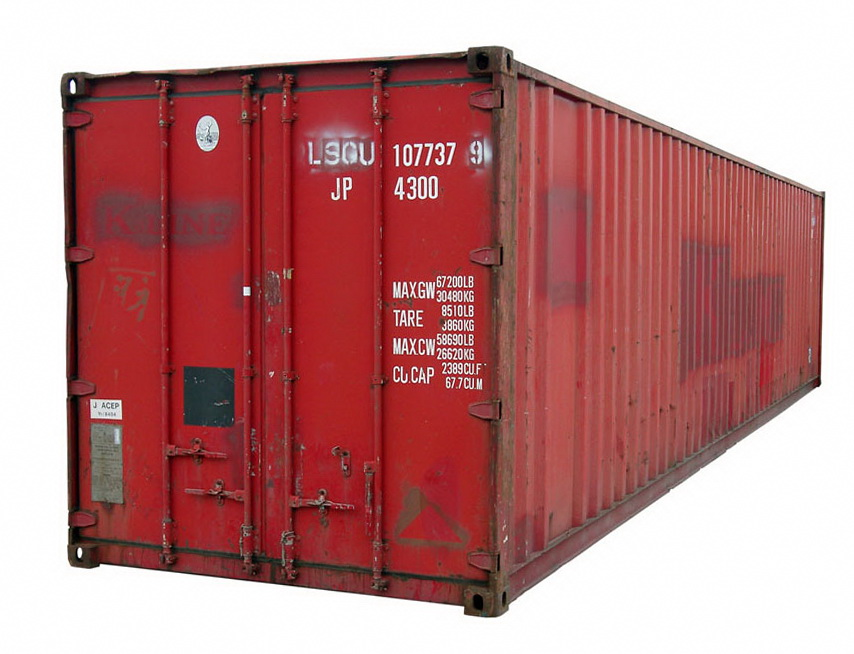
\includegraphics[width=0.7\textwidth]{images/shipping_container}
\end{frame}

\begin{frame}{Before Containerization}
\begin{columns}[c]
\begin{column}{0.5\textwidth}
\begin{itemize}
\item Goods had to be loaded and unloaded individually
\item Inefficient - it was not uncommon to spend more time loading and loading goods than transporting them
\item Insecure - goods had be handled by many people, increasing the chance for loss and theft
\item Inaccessible - Long distance shipping only available to the wealthy 
\end{itemize}
\end{column}
\begin{column}{0.5\textwidth}
\centering
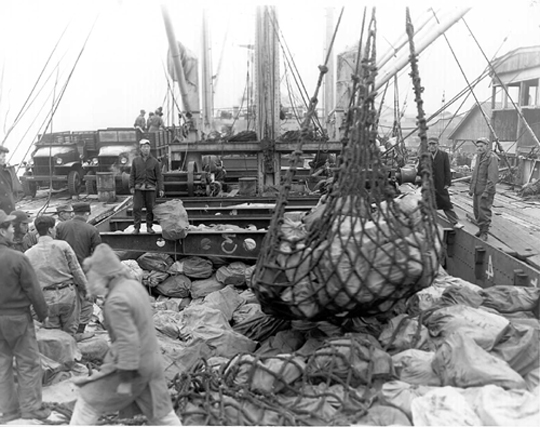
\includegraphics[width=0.85\textwidth]{images/old_ship_unloading}
\end{column}
\end{columns}
\end{frame}

\begin{frame}{After Containerization}
\begin{columns}[c]
\begin{column}{0.5\textwidth}
\begin{itemize}
\item Standardized - containers are all the same size and weight allowances
\item Efficient - containers are easy to load and unload and transfer to other modes of transportation
\item Secure - goods may be secured in containers from source to final destination
\item Available - cost effective to ship goods across the world
\end{itemize}
\end{column}
\begin{column}{0.5\textwidth}
\centering
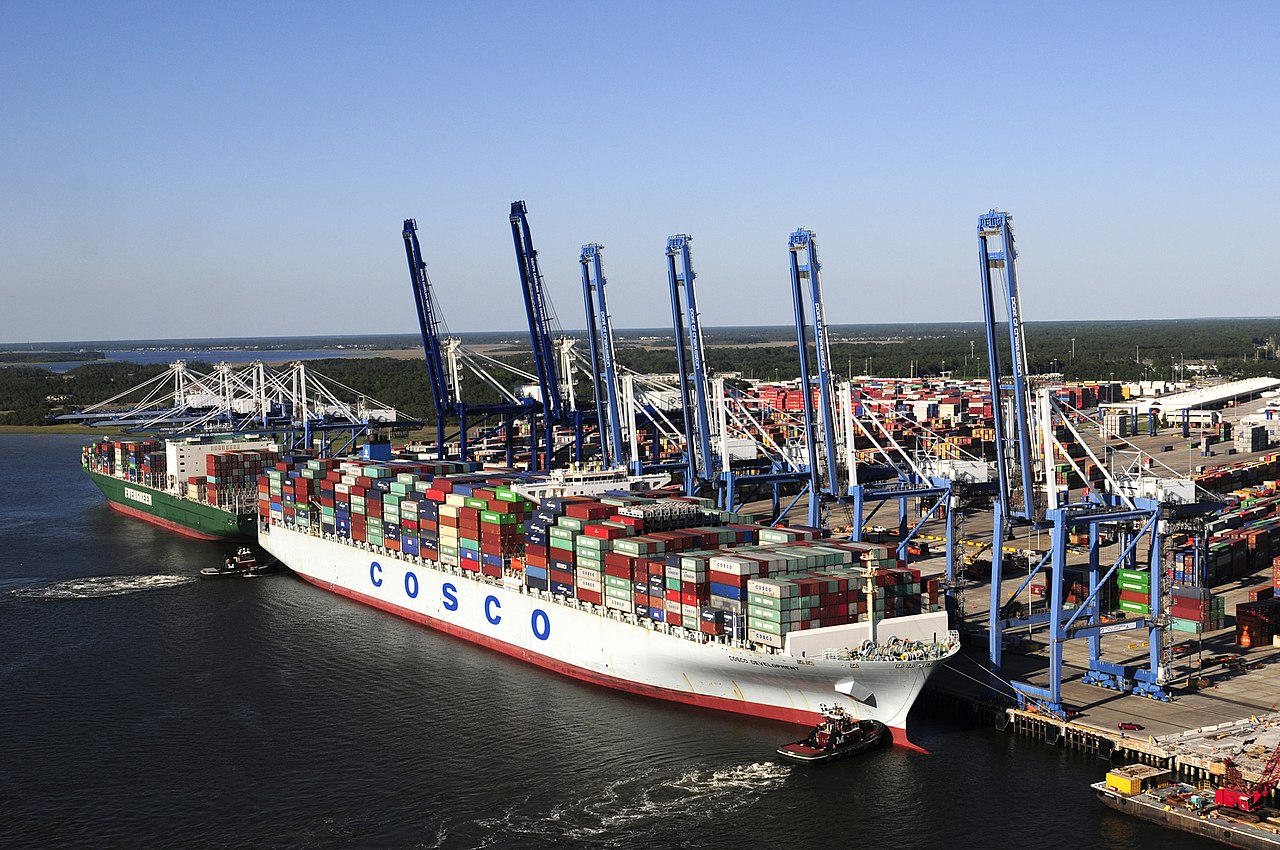
\includegraphics[width=0.85\textwidth]{images/cargo_ship}
\end{column}
\end{columns}

\end{frame}

\begin{frame}{Common Issues with Software Stacks}
\begin{itemize}
\item My software doesn’t build on this system...
\item I’m missing dependencies...
\item I need version 1.3.2 but this system has version 1.0.2..
\item I need to re-run the exact same thing 12 months from now...
\item I want to run this exact same thing somewhere else...
\item I want my collaborators to have the same exact software as me...
\item I’ve heard about these Containers, can I just run that?
\item Can I run docker on this HPC system?
\end{itemize}
\end{frame}

\begin{frame}{What about computing?}
\begin{itemize}
\item It's common to run on multiple systems with different requirements
\item We would like to avoid installing the same sets of software again and again
\item We would like other people to run our software without our help
\item We would like to preserve a known configuration that our software works in
\end{itemize}
\end{frame}

\begin{frame}{Possible Solution: Containers}
\begin{itemize}
\item What are Containers?
\item Uses a combination of Kernel ``cgroups'' and ``namespaces'' to create isolated environments
\item Long history of containers Solaris Zones (2005), LXC(2008), LMCTFY/Google and then Docker(2013).
\item Entire ecosystem has grown around containers including open standards and governance.
\end{itemize}
\end{frame}

\begin{frame}{Possible Solution: Containers}
\begin{itemize}
\item A lightweight collection of executable software that encapsulates
everything needed to run an application
\begin{itemize}
\item Minus the OS kernel
\item Based on Linux only
\end{itemize}
\item Processes and all user-level software is isolated
\item Creates a portable* software ecosystem
\item Think \mintinline{sh}{chroot} on steroids
\item Docker is the most common tool today
\begin{itemize}
\item Available on all major platforms
\item Widely used in industry
\item Integrated container registry via Dockerhub
\end{itemize}
\end{itemize}
\end{frame}

\begin{frame}{Containers Overview}
\begin{itemize}
\item Containers offer the ability to run fully customized software stacks,
\textit{e.g.} based on different Linux distributions and versions
\item Containers are not virtual machines, where an entire hardware platform is
virtualized, rather containers share a common kernel and access to physical
hardware resources
\end{itemize}
\end{frame}

\begin{frame}{Hypervisors and Containers}
\begin{itemize}
\item Type 1 hypervisors insert layer below host OS
\item Type 2 hypervisors work as or within the host OS
\item Containers do not abstract hardware, instead provide ``enhanced chroot'' to
create isolated environment using a common kernel
\item Location of abstraction can have impact on performance
\item All enable custom software stacks on existing hardware
\end{itemize}
\end{frame}

\begin{frame}{Hypervisors and Containers}
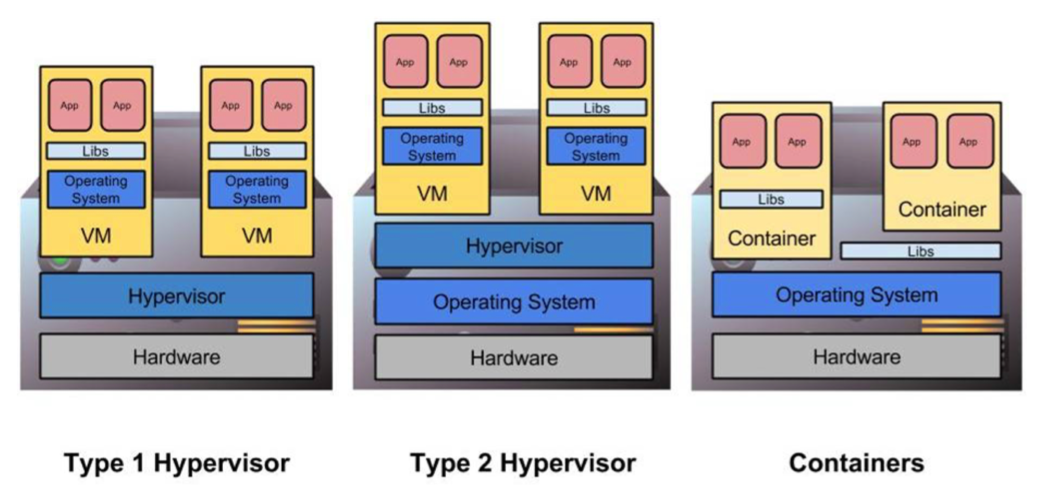
\includegraphics[height=0.8\textheight]{images/hypervisors_vs_containers.png}
\end{frame}

\begin{frame}{Container Benefits}
\begin{description}
\item[Performant] Containers can perform at near native performance.
\item[Flexible] Install (almost) any software you need.
\item[Reproducible] Define complex software environments that are verifiable.
\item[Compatible] Built on open standards that works on all major Linux distributions.
\item[Portable] Build once and run (almost) anywhere.
\end{description}
\end{frame}

\begin{frame}{Container Limitations}
\begin{description}
\item[Hardware] Containers are limited to the same CPU architecture
(x86\_64, ARM, Power, etc.) and binary formats
\item[Software] Requires glibc and kernel compatibility between host and
container. Other kernel level APIs may also need to be compatible (e.g.
CUDA/GPU drivers, network drivers, etc.)
\item[Filesystem] Paths can be different when viewed from inside or outside of
a container
\end{description}
\end{frame}

\begin{frame}{Nomenclature}
\begin{description}
\item[Image] A read-only template that defines how to create a container
\item[Container] An instantiation of an image, a running instance
\item[Container Runtime] Tool or service to execute and manage containers
\item[Registry] A service that is used to store and distribute images
\end{description}
\end{frame}

\begin{frame}{Docker and HPC}
\begin{itemize}
\item We don't allow direct Docker use on SMU HPC systems
\item Docker's security model is designed to support users "trusted" users running "trusted" containers (e.g. users who can escalate to root access)
\item Docker is not designed to support scripted / batch based workflows
\item Docker is not designed to support parallel applications
\end{itemize}
\end{frame}

\begin{frame}{Apptainer/Singularity Features}
\begin{itemize}
\item Containers are a single image file
\item No root owned daemon processes
\item User inside containers are the same as users outside the container (no contextual changes)
\item Supports shared, multi-user environments
\item Supports HPC hardware such as GPUs and Infiniband networks
\item Supports HPC applications like MPI
\end{itemize}
\end{frame}

\begin{frame}{Common Use Cases}
\begin{itemize}
\item Converting Docker containers to Apptainer/Singularity
\item Building and running software that require newer systems and libraries 
\item Running commercial software binaries that have specific requirements
\end{itemize}
\end{frame}



\section{Docker}

\begin{frame}{Dockerfile}
\begin{itemize}
\item Is a ``recipe'' for how to construct an image.
\item Starts \mintinline{sh}{FROM} a defined base image.
\item Several basic commands (\mintinline{sh}{ADD}, \mintinline{sh}{COPY},
\mintinline{sh}{RUN}, etc.) can be applied to mutate the image to the desired
state.
\item Metadata labels can also be added to provide information about the image.
\item In addition to the file system changes, the Dockerfile can also control
settings like the environment, the starting directory, and default commands.
\end{itemize}
\end{frame}

\begin{frame}{Basic Dockerfile}
\inputminted{Dockerfile}{src/python3.dockerfile}
\end{frame}

\begin{frame}{Docker Image Registries}
\begin{itemize}
\item There are several public and private sources for Docker images.
\item Images can be used as the base image for custom images.
\item Already optimized images can help with reproducible and efficient
development workflows.
\end{itemize}
\end{frame}

\begin{frame}{Docker Image Registries}
\begin{description}
\item[Docker] \url{https://hub.docker.com}
\item[GitHub Packges] \url{https://github.com/features/packages}
\item[Quay.io] \url{https://quay.io}
\item[NVIDIA] \url{https://catalog.ngc.nvidia.com}
\item[Intel] \url{https://hub.docker.com/u/intel}
\item[AMD] \url{https://hub.docker.com/u/amdih}
\end{description}
\end{frame}

\begin{frame}{Pulling Images from Registries}
\inputminted{sh}{src/docker_image_registries.sh}
\end{frame}

\begin{frame}{Multi-Architecture Builds}
\begin{itemize}
\item Images are CPU-architecture specific
\item Docker supports multi-architecture builds
\begin{itemize}
\item Platforms: amd64, arm32v5, arm32v6, arm32v7, arm64v8, i386, ppc64le, and s390x
\item \mintinline{sh}{docker build --platform } with single platform
\item \mintinline{sh}{docker buildx --platform } with list of platforms
\end{itemize}
\item Builds on non-native platforms will be slower as it is running via
emulation
\end{itemize}
\end{frame}

\begin{frame}{Docker Multi-Architecture Builds}
\inputminted{sh}{src/docker_buildx.sh}
\end{frame}

\begin{frame}{Multi-Stage Builds with Docker}
\begin{itemize}
\item Images with build tools can be very large.
\item Use the needed image for building.
\item Use the smallest image for running.
\item Define both the build and execution in a single Dockerfile.
\end{itemize}
\end{frame}

\begin{frame}{Basic Multi-Stage Dockerfile}
\inputminted{Dockerfile}{src/hello_world.dockerfile}
\end{frame}

\begin{frame}{Docker Multi-Architecture Builds}
\inputminted{sh}{src/docker_build_multi.sh}
\end{frame}

\section{Apptainer/Singularity}

\begin{frame}{Building Apptainer/Singularity Images}
\begin{itemize}
\item Singularity has it's own image
\href{https://sylabs.io/guides/3.7/user-guide/definition_files.html}{definition
language}.
\begin{itemize}
\item Requires (re)writing the definition file.
\item Requires root or ``fakeroot'', which is not widely available on HPC
systems.
\item Can be done on a Linux system with Singularity installed and them copying
the image.
\item Not generally recommended as there would be two definition files to
maintain, presumably Docker and also Singularity.
\end{itemize}
\item Pull from Docker registries.
\begin{itemize}
\item Requires pushing and pulling of Docker images.
\end{itemize}
\item Build from Docker archives.
\begin{itemize}
\item Requires exporting, copying, and conversion of Docker images.
\end{itemize}
\end{itemize}
\end{frame}

\begin{frame}{Pulling Docker Containers}
\inputminted[firstline=0, lastline=8]{sh}{src/docker_buildx_singularity.sh}
\end{frame}

\begin{frame}{Pulling Docker Containers}
\inputminted[firstline=10]{sh}{src/docker_buildx_singularity.sh}
\end{frame}

\begin{frame}{Singularity Workflow}
\begin{itemize}
\item Build your Singularity containers on a local system you have root or sudo access. Alternatively build a Docker container
\item Transfer your container to the HPC system. If you used Docker, you will need to convert the image 
\item Run your Singularity containers
\end{itemize}
\end{frame}

\begin{frame}{Converting from Docker Archives}
\inputminted[firstline=15, lastline=20]{sh}{src/build_python3_docker.sh}
\end{frame}

\begin{frame}{Full Example Workflow}
\begin{itemize}
\item Build application, separating build and deployment containers
\item Script container image build and make Lmod module file for ease of use
\item Convert Docker image to Apptainer/Singularity image using the docker2singularity tool
\end{itemize}
\end{frame}

\begin{frame}{Full Example Workflow}
\inputminted[firstline=1, lastline=18]{Dockerfile}{src/molden/Dockerfile}
\end{frame}

\begin{frame}{Full Example Workflow}
\inputminted[firstline=20, lastline=32]{Dockerfile}{src/molden/Dockerfile}
\end{frame}

\begin{frame}{Full Example Workflow}
\inputminted[firstline=34, lastline=48]{Dockerfile}{src/molden/Dockerfile}
\end{frame}

\begin{frame}{Full Example Workflow}
\inputminted[firstline=1, lastline=11]{sh}{src/molden/build_images.sh}
\end{frame}

\begin{frame}{Full Example Workflow}
\inputminted[firstline=13, lastline=21]{sh}{src/molden/build_images.sh}
\end{frame}

\begin{frame}{Full Example Workflow}
\inputminted[firstline=23, lastline=28]{sh}{src/molden/build_images.sh}
\end{frame}

\begin{frame}{Full Example Workflow}
\inputminted[firstline=30, lastline=34]{sh}{src/molden/build_images.sh}
\end{frame}

\begin{frame}{Full Example Workflow}
\inputminted[firstline=36, lastline=43]{sh}{src/molden/build_images.sh}
\end{frame}

\begin{frame}{Full Example Workflow}
\inputminted[firstline=1, lastline=5]{lua}{src/molden/molden.lua}
\end{frame}

\begin{frame}{Full Example Workflow}
\inputminted[firstline=7, lastline=15]{lua}{src/molden/molden.lua}
\end{frame}

\begin{frame}{Full Example Workflow}
\inputminted[firstline=17, lastline=28]{lua}{src/molden/molden.lua}
\end{frame}

\section{Spack}

\begin{frame}{Spack Containerize}
\begin{itemize}
\item Build images defined by Spack environments.
\item Spack-based build optimizations are preserved.
\item Intermediate Dockerfile uses multi-stage builds
\item Currently does not work for multi-architecture builds.
\end{itemize}
\end{frame}

\begin{frame}{Define a Spack Environment}
\inputminted{yaml}{src/spack.yaml}
\end{frame}

\begin{frame}{Build the Image from the Environment}
\inputminted{sh}{src/spack_containerize.sh}
\end{frame}

\section{Kubernetes}

\begin{frame}{What is Kubernetes}
\begin{itemize}
\item Platform for managing containerized workloads and services
\begin{itemize}
\item Portable
\item Extensible
\item Open Source
\item Originally developed by Google for managing service deployment
\end{itemize}
\item Kubernetes (K8s)
\begin{itemize}
\item Kubernetes, from Greek, means helmsman or pilot
\item ``K8s'' comes from the 8 characters between the ``k'' and the ``s''
\end{itemize}
\end{itemize}
\end{frame}

\begin{frame}{Benefits of Kubernetes}
\begin{itemize}
\item Persistence
\item Load balancing
\item Self-healing
\item Automated rollouts and rollbacks
\item Resource optimization
\item Infrastructure as code
\end{itemize}
\end{frame}

\begin{frame}{Application Deployment Scenarios}
\centering
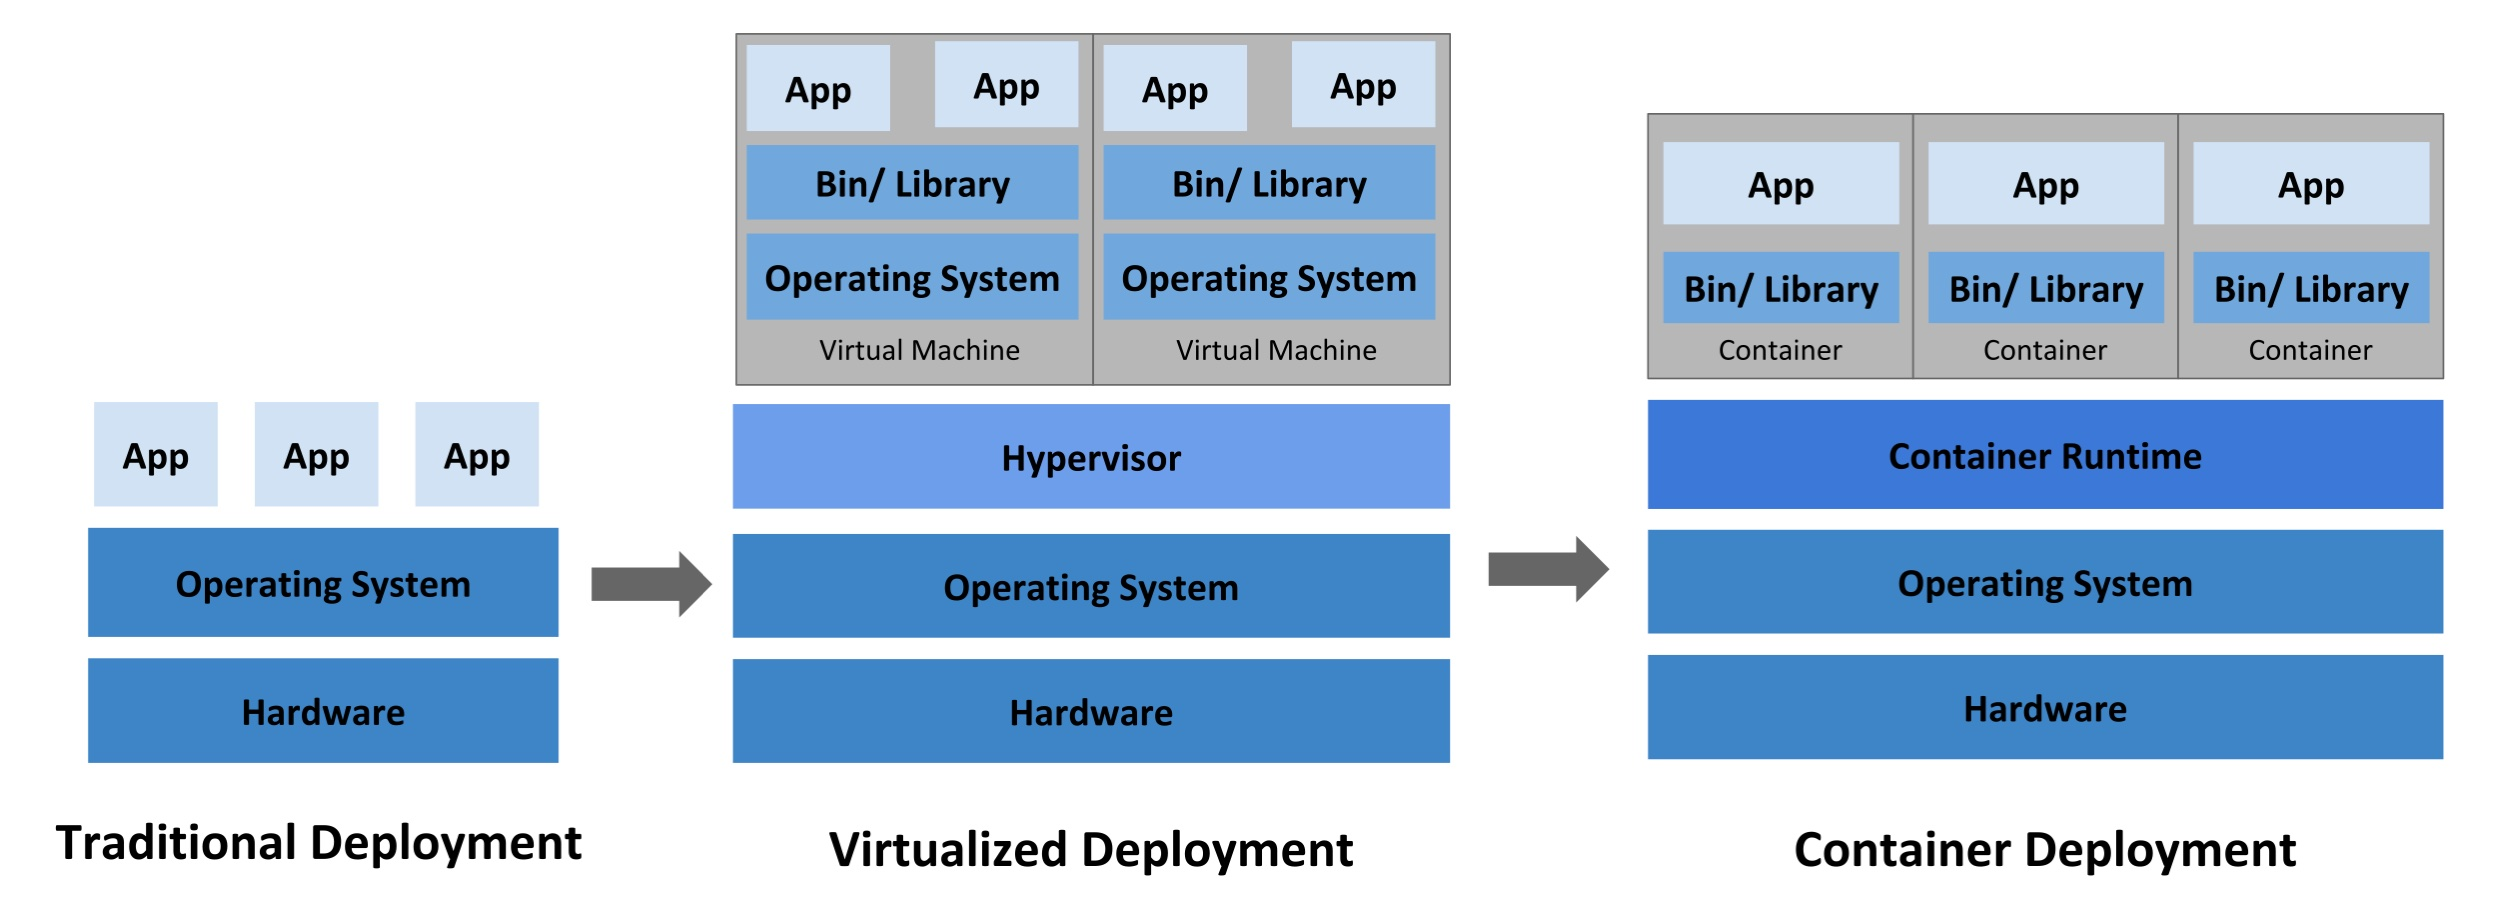
\includegraphics[height=0.7\textheight]{images/deployment_types.jpg}
\end{frame}

\begin{frame}{K8s Cluster Components}
\centering
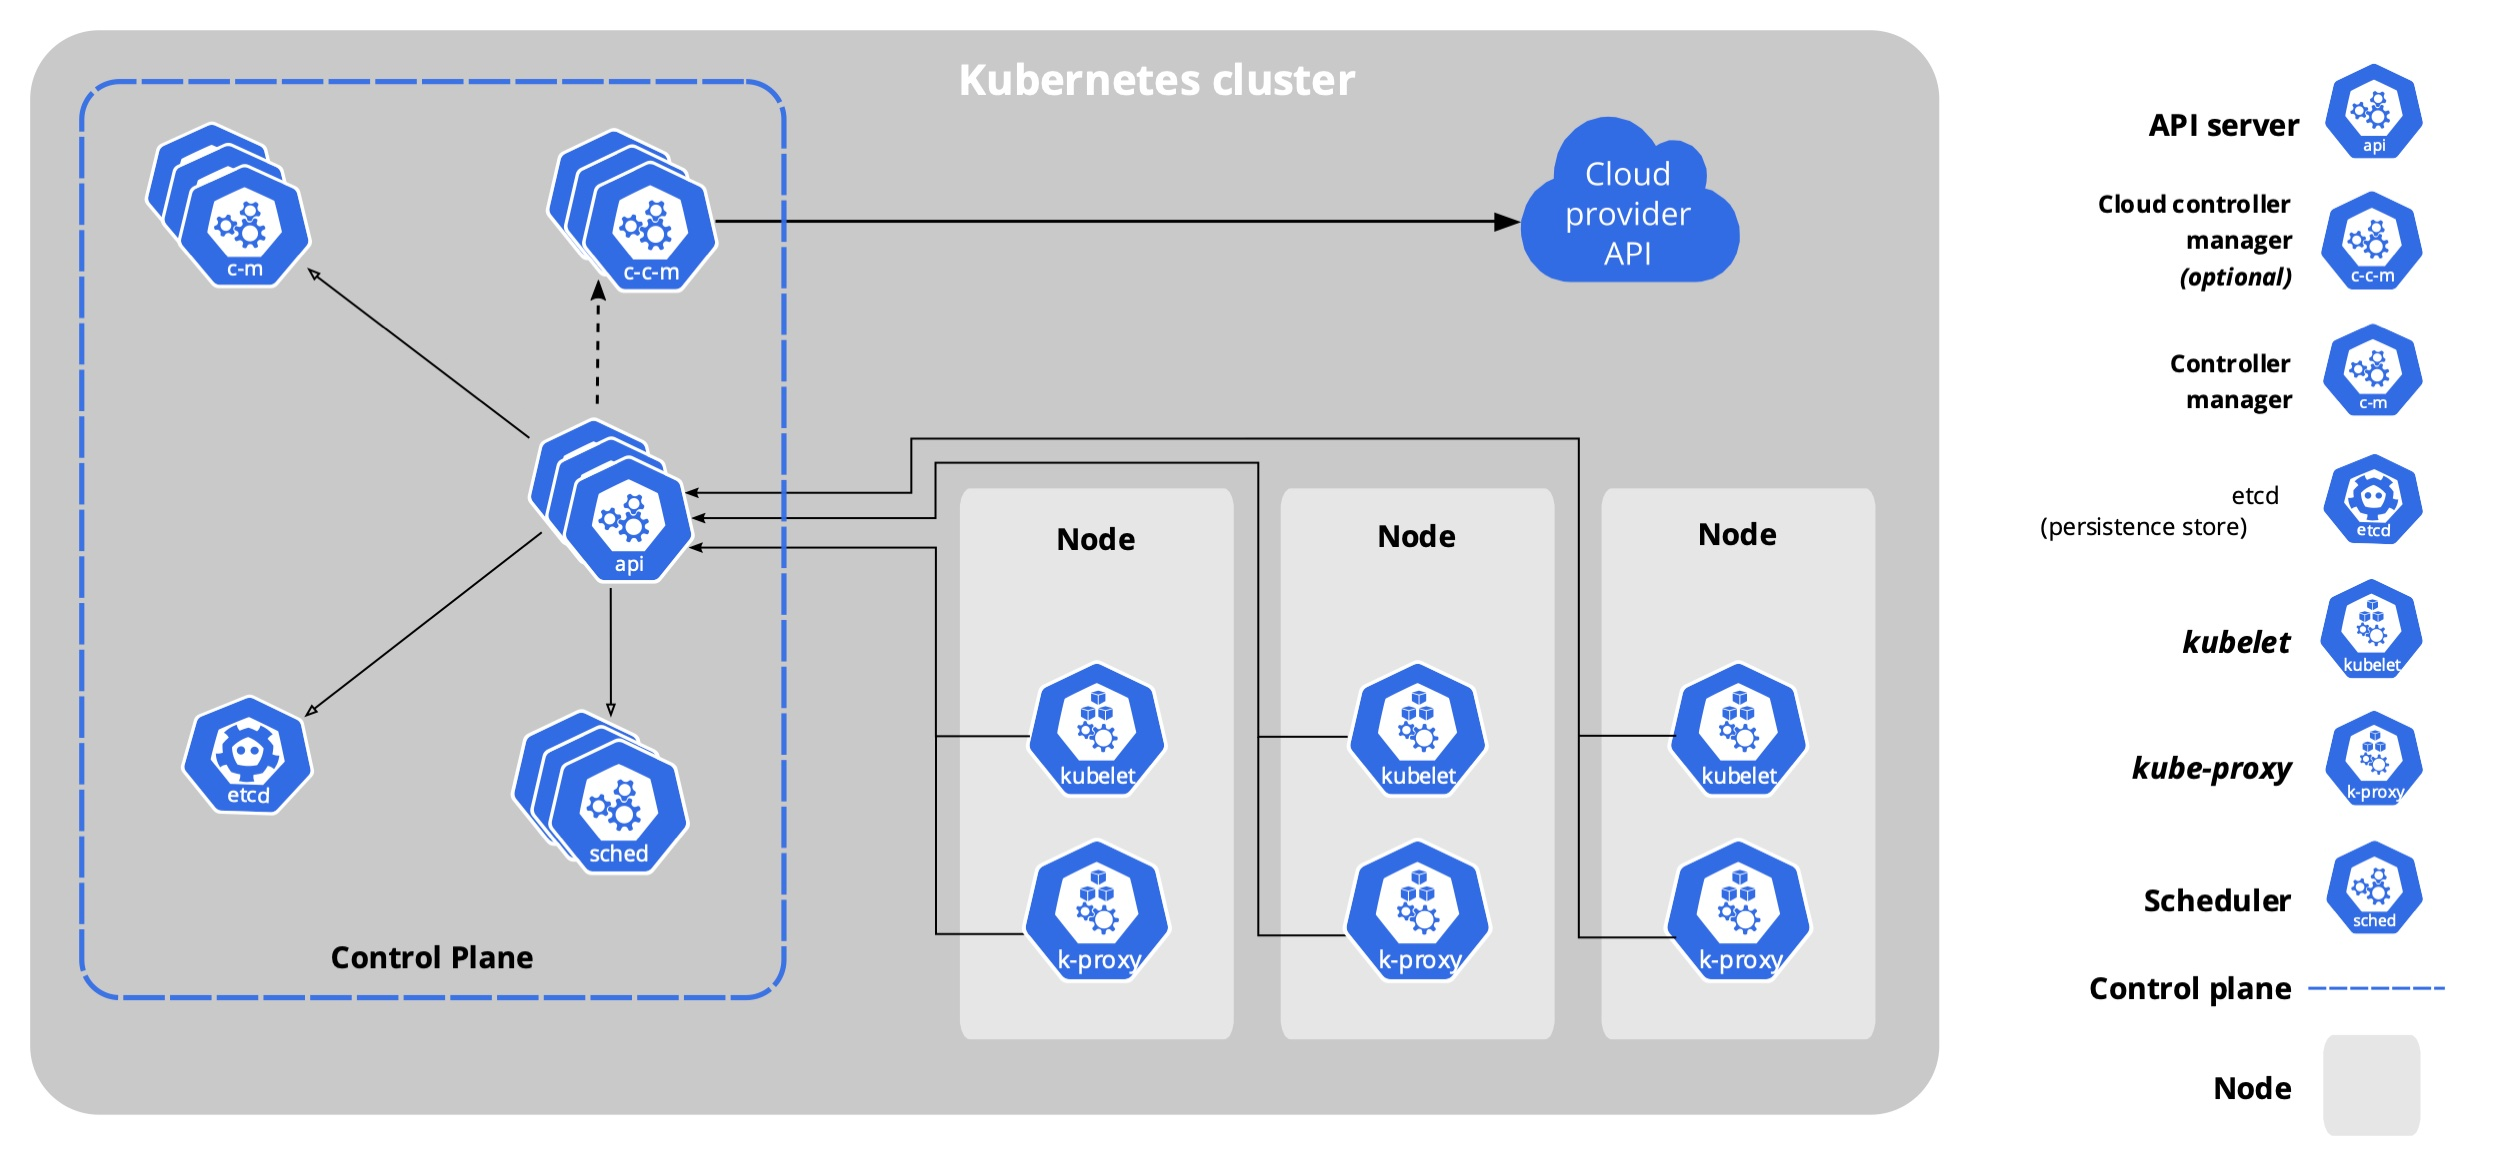
\includegraphics[height=0.7\textheight]{images/k8s_cluster.jpg}
\end{frame}

\begin{frame}{Kubernetes Distributions}
\scriptsize
\begin{columns}[c]
\begin{column}{0.5\textwidth}
\begin{itemize}
\item kubeadm
\item Minikube
\begin{itemize}
\item Local K8s clusters on macOS, Linux, and Windows
\item Commonly used for developing applications
\end{itemize}
\item K3s
\item GKE (Google Kubernetes Engine)
\item AKS (Microsoft Azure Kubernetes Services)
\item EKS (Amazon Elastic Kubernetes Service)
\item RKE (SUSE Rancher Kubernetes Engine)
\item Ubuntu
\begin{itemize}
\item Charmed Kubernetes
\item MicoK8s 
\end{itemize}
\end{itemize}
\end{column}
\begin{column}{0.5\textwidth}
\centering

\includegraphics[width=0.85\textwidth]{images/k8s_distributions.jpg}
\end{column}
\end{columns}
\end{frame}

\begin{frame}{Pods}
\begin{itemize}
\item Job definition
\begin{itemize}
\item One or more containers
\item Specification on how to run them
\end{itemize}
\item Shared resources
\begin{itemize}
\item Compute
\item Storage
\item Networking
\item Context
\begin{itemize}
\item Location and scheduling
\end{itemize}
\end{itemize}
\end{itemize}
\end{frame}

\begin{frame}{Types of Workloads}
\begin{description}
\item[Deployments] Manage changes to running Pods as specified rate
\item[ReplicaSet] Specify the number of available and identical Pods for high-availability
\item[StatefulSets] Deployment of Pods with a specific ordering, e.g. Pods with unique network IDs 
\item[DaemonSets] Every node gets a Pod, which dynamically changes as the cluster size changes
\item[Jobs] Batch scheduling of workloads (similar to Slurm Arrays, but with redundancy)
\item[Cronjobs] Scheduled workloads
\end{description}
\end{frame}

\begin{frame}{Pod Security}
\begin{itemize}
\item Specify the Pod level of isolation
\item Pod Security Standards
\begin{itemize}
\item Privileged (allows for privilege escalation)
\item Baseline (prevents privilege escalation)
\item Restricted (hardened security)
\begin{itemize}
\item Security-critical applications
\item Low-trust users
\end{itemize}
\end{itemize}
\item Levels of enforcement
\begin{itemize}
\item Enforce
\item Audit (log annotation)
\item Warn (user-facing warning)
\end{itemize}
\end{itemize}
\end{frame}



\begin{frame}{Help?}
\centering
Need help or have questions?\\
\href{mailto:rkalescky@smu.edu}{rkalescky@smu.edu} \\
\href{mailto:jlagrone@smu.edu}{jlagrone@smu.edu} \\
\href{mailto:help@smu.edu}{help@smu.edu}  (include HPC in the subject line)
\end{frame}



\end{document}

